\chapter{Results}

	\section{Comparative analyses of super-enhancers reveal conserved elements in vertebrate genomes}

		Super-enhancers are regulatory hubs with main roles in the control of cell identity. Extensive research of super-enhancers in mammalian genomes have highlighted their impact in the initiation and maintenance of transcription and in the 3D genome organization. Nevertheless, it was unknown if regions identified in non-mammalian organisms following the same criteria used to identify super-enhancers in mammals did represented regions with equivalent functionalities. To gain insight into this possibility, super-enhancers were annotated in the zebrafish genome and their features compared to those of mouse and human super-enhancers.\\

		\subsection{Main findings}

			For this study, super-enhancers annotations were generated based on H3K27ac ChIP-seq signal enrichment in four tissues and pluripotent cells in zebrafish, mouse and human. Similar to mammalian super enhancers, zebrafish super-enhancers are longer than the regions annotated as typical enhancers, however, differences in the genomic distribution of super-enhancers were observed. Whereas mammalian super-enhancers are preferentially distributed in TSS downstream regions and enriched over gene bodies, no clear tendency in the distribution of super-enhancers was characterized in zebrafish.\\

			High cell- and tissue-specificity was identified as an additional commonality between mammalian and zebrafish super-enhancers based on the comparison of intersecting super-enhancer regions in zebrafish. Indeed, the proportion of regions that are annotated as super-enhancers in all cells and tissues analyzed is lower than the proportion corresponding to typical enhancers. In addition, GO analysis of super-enhancers show enriched terms associated with relevant processes or functions of each cell type and tissue.\\

			Sequence conservation analysis of constitutive regions within super-enhancers and typical enhancers of zebrafish, mouse and human indicates no significant higher sequence conservation of super-enhancer constituents in general. Nevertheless, a set of orthologous genes located in close proximity to super-enhancers in the three species was identified. The super-enhancers associated to those genes show higher sequence conservation than those without orthologous associations in zebrafish, mouse and human.\\

			To test the contribution to super-enhancer function of different regions within them, two super-enhancers were dissected using enhancer reporter assays. Of note, regions with equivalent functions in zebrafish and mouse for both super-enhancers were identified through this analysis. One of the regions that was identified likely corresponds to a shadow enhancer given its lack of H3K27ac enrichment and accessibility signal.\\

			Altogether, these results confirm super-enhancers as conserved regulators throughout vertebrate evolution and epitomize the importance of analyzing enhancer clusters as a unit. The latter, reasoning that identification of super-enhancers can be used as an strategy to characterize functionally conserved elements and to understand redundancy of transcriptional regulation.\\

		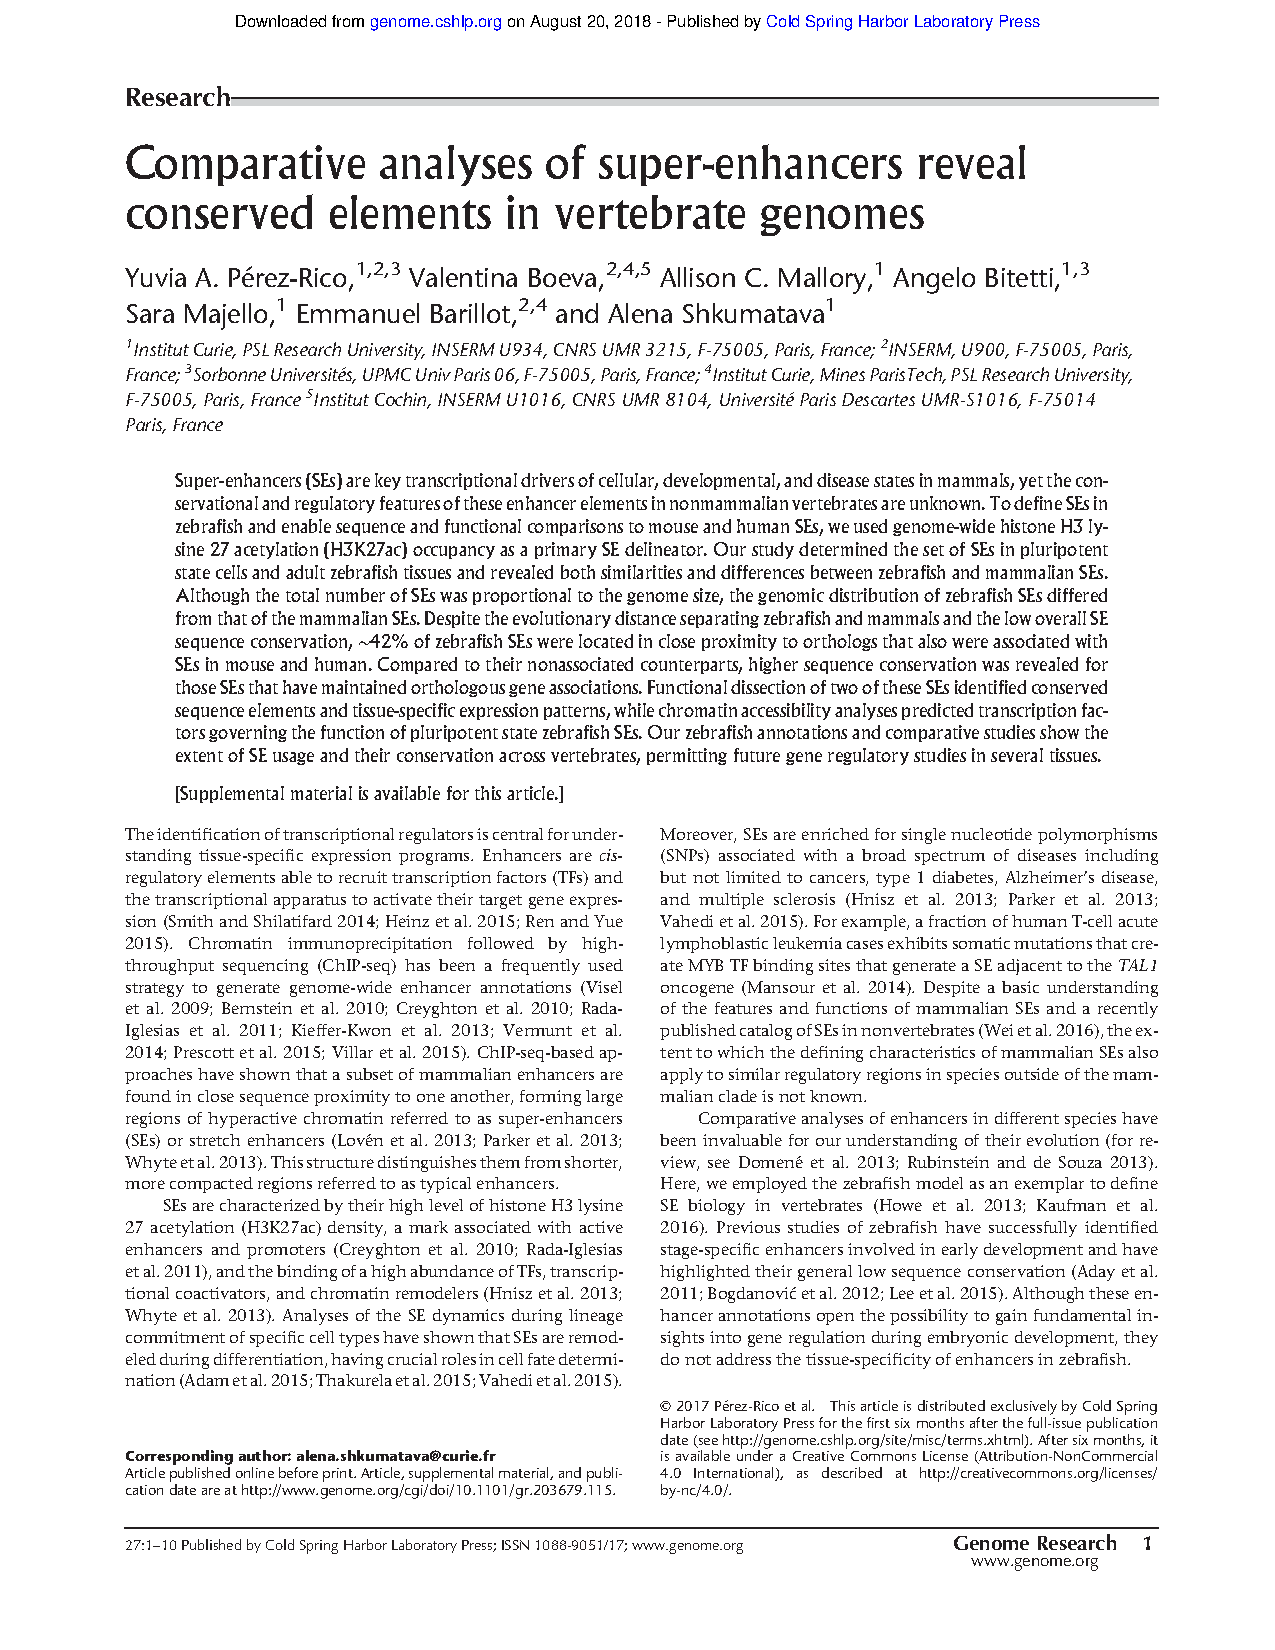
\includepdf[pages=-, pagecommand={\thispagestyle{plain}}, scale=0.95]{GenomeRes_2017/Genome_Res_2017.pdf}

		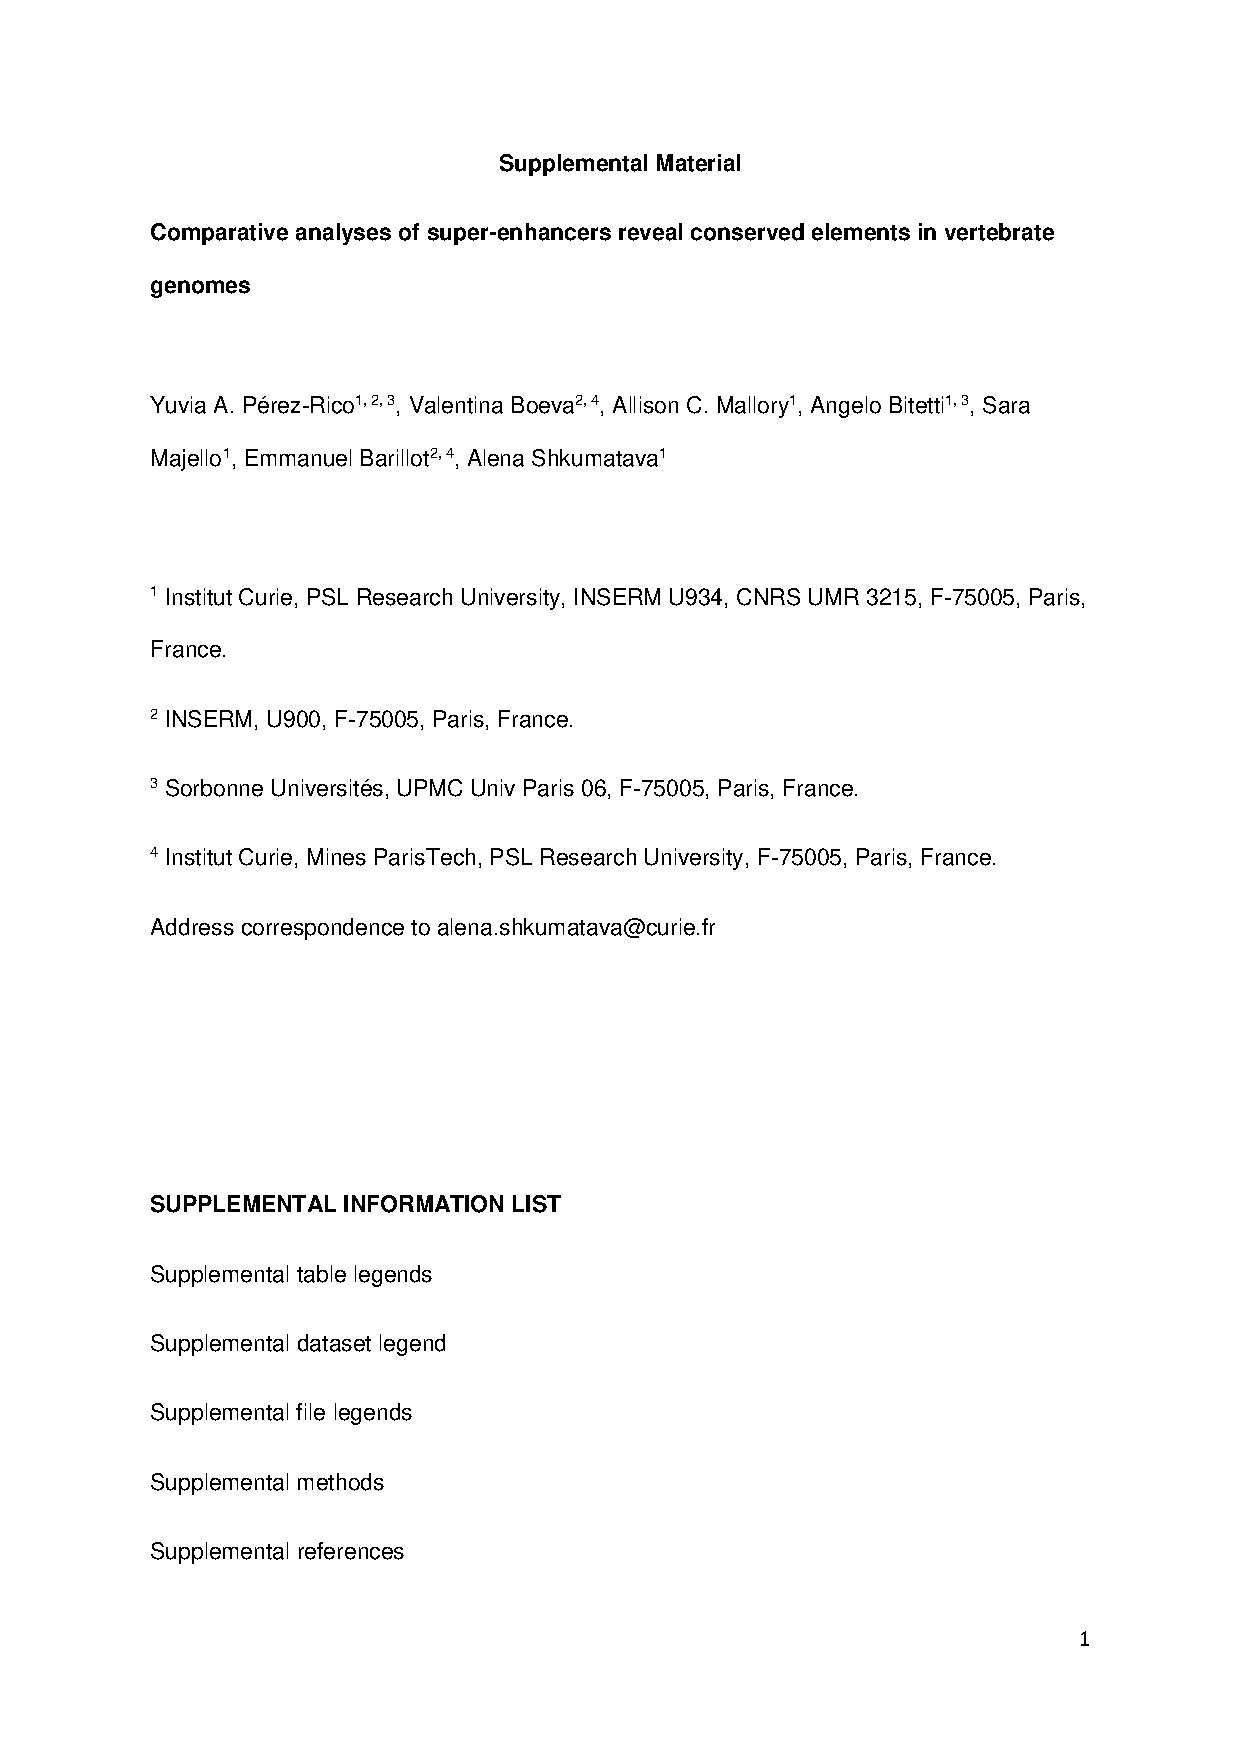
\includepdf[pages=-, pagecommand={\thispagestyle{plain}}, scale=0.9]{GenomeRes_2017/Supplemental_Material.pdf}

		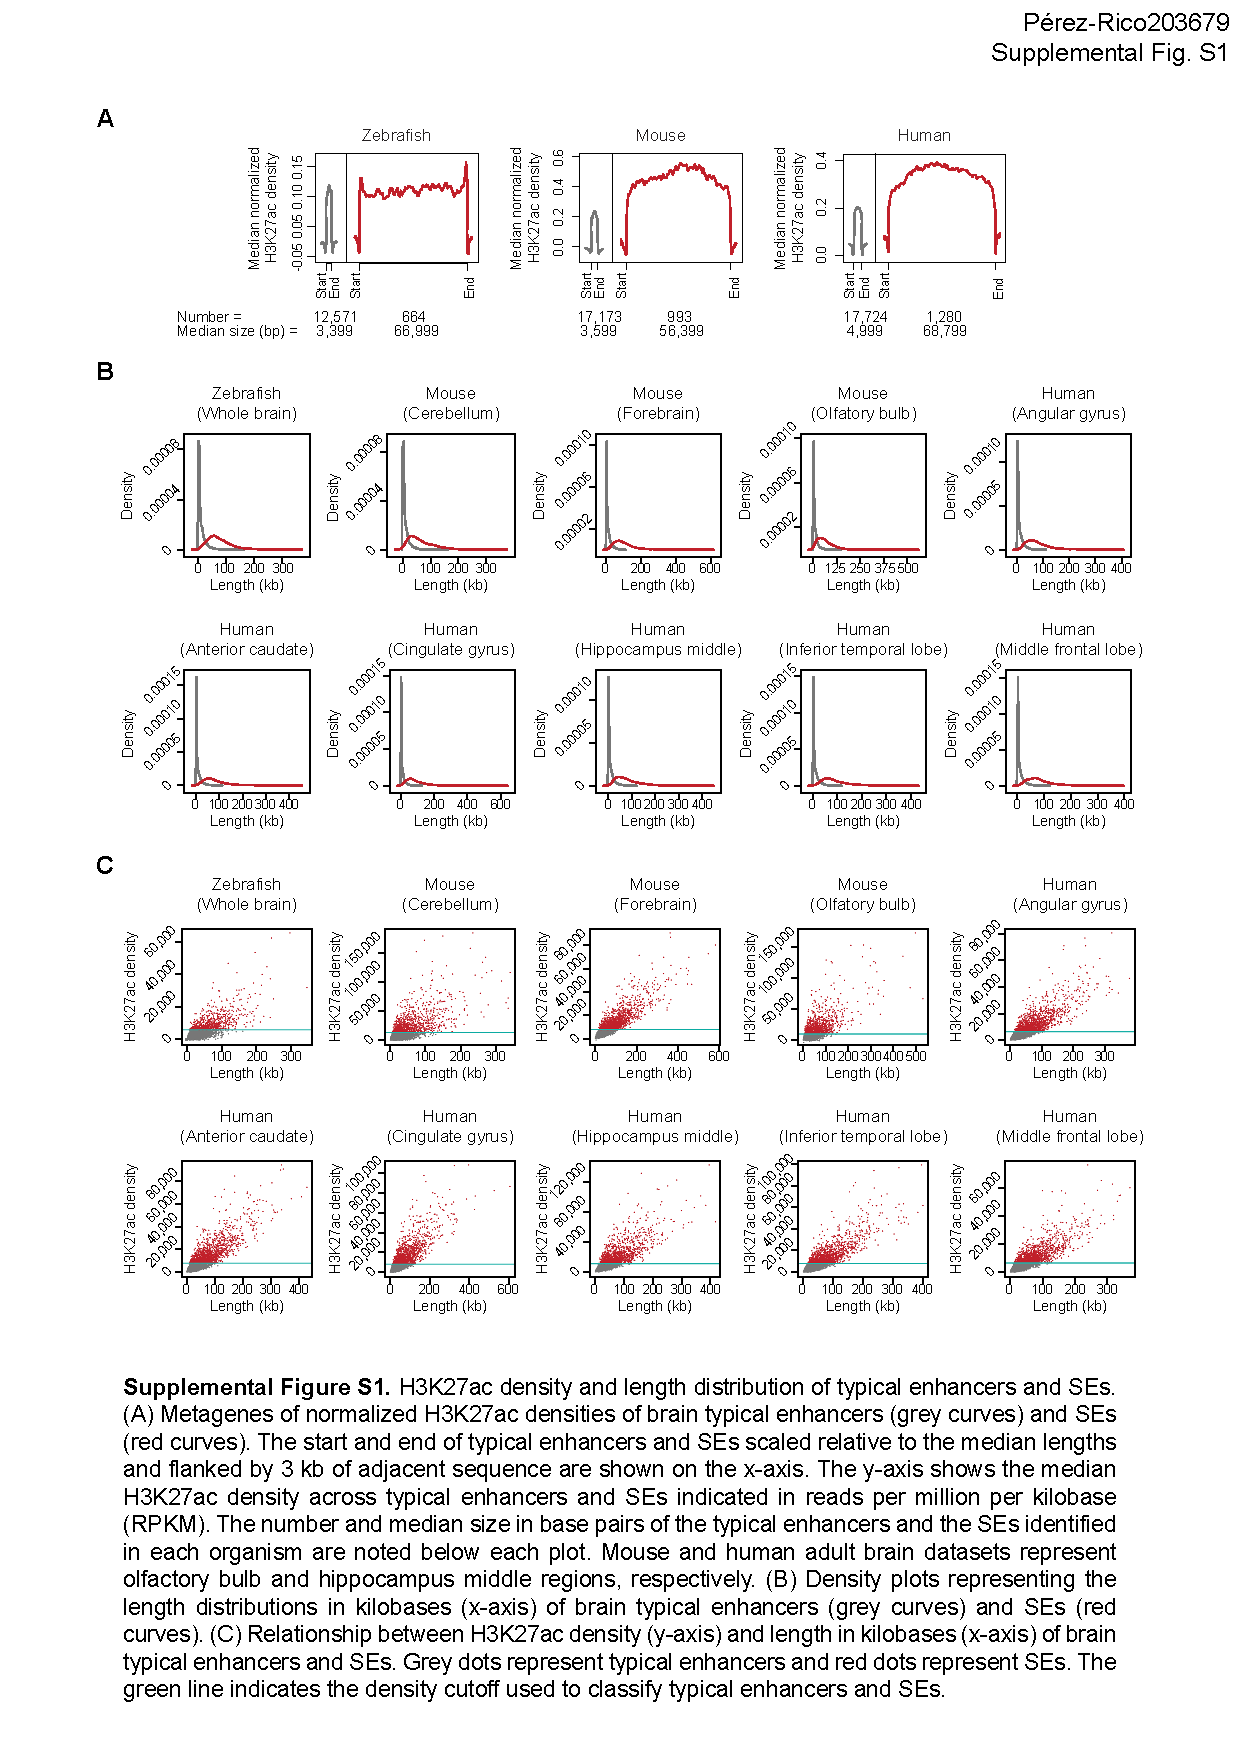
\includepdf[pages=-, pagecommand={\thispagestyle{plain}}, scale=0.8]{GenomeRes_2017/Supplemental_Fig_S1.pdf}

		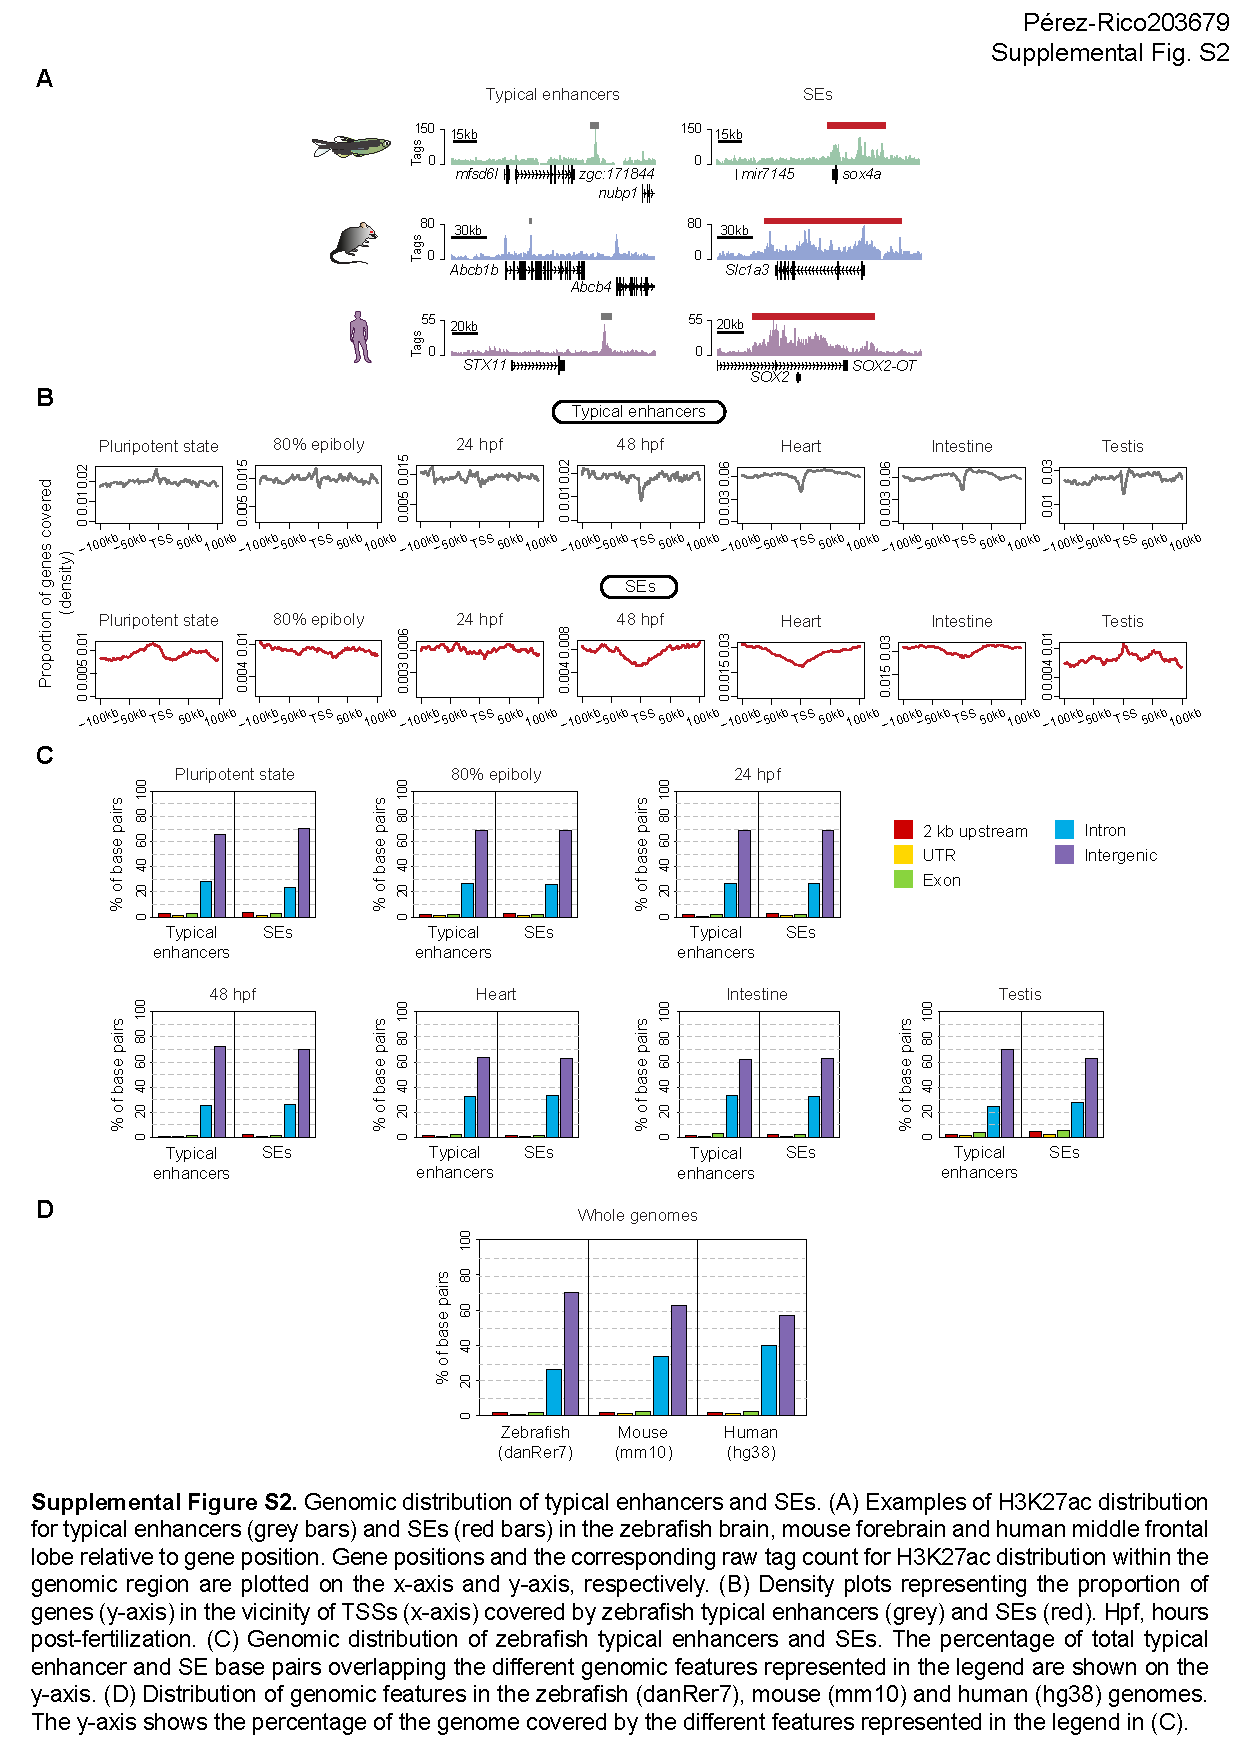
\includepdf[pages=-, pagecommand={\thispagestyle{plain}}, scale=0.8]{GenomeRes_2017/Supplemental_Fig_S2.pdf}

		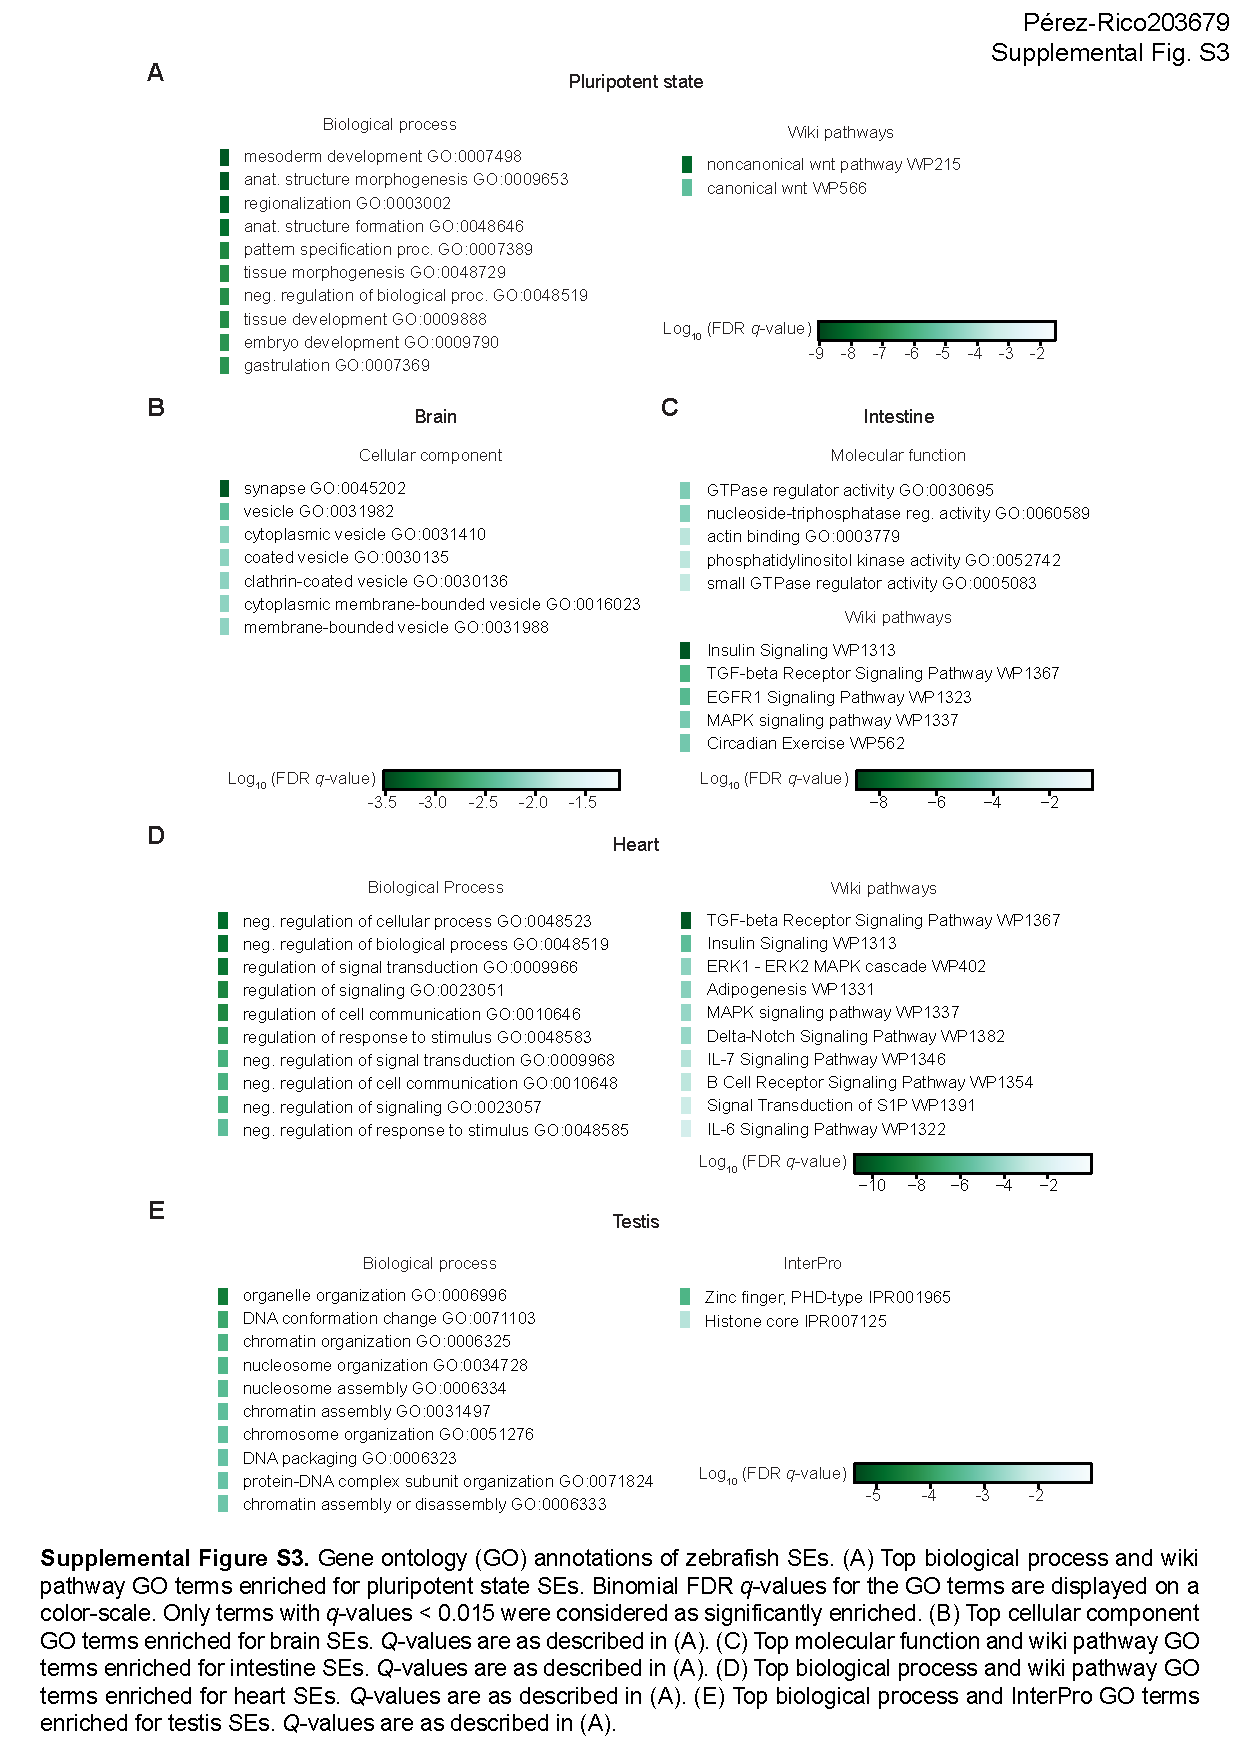
\includepdf[pages=-, pagecommand={\thispagestyle{plain}}, scale=0.8]{GenomeRes_2017/Supplemental_Fig_S3.pdf}

		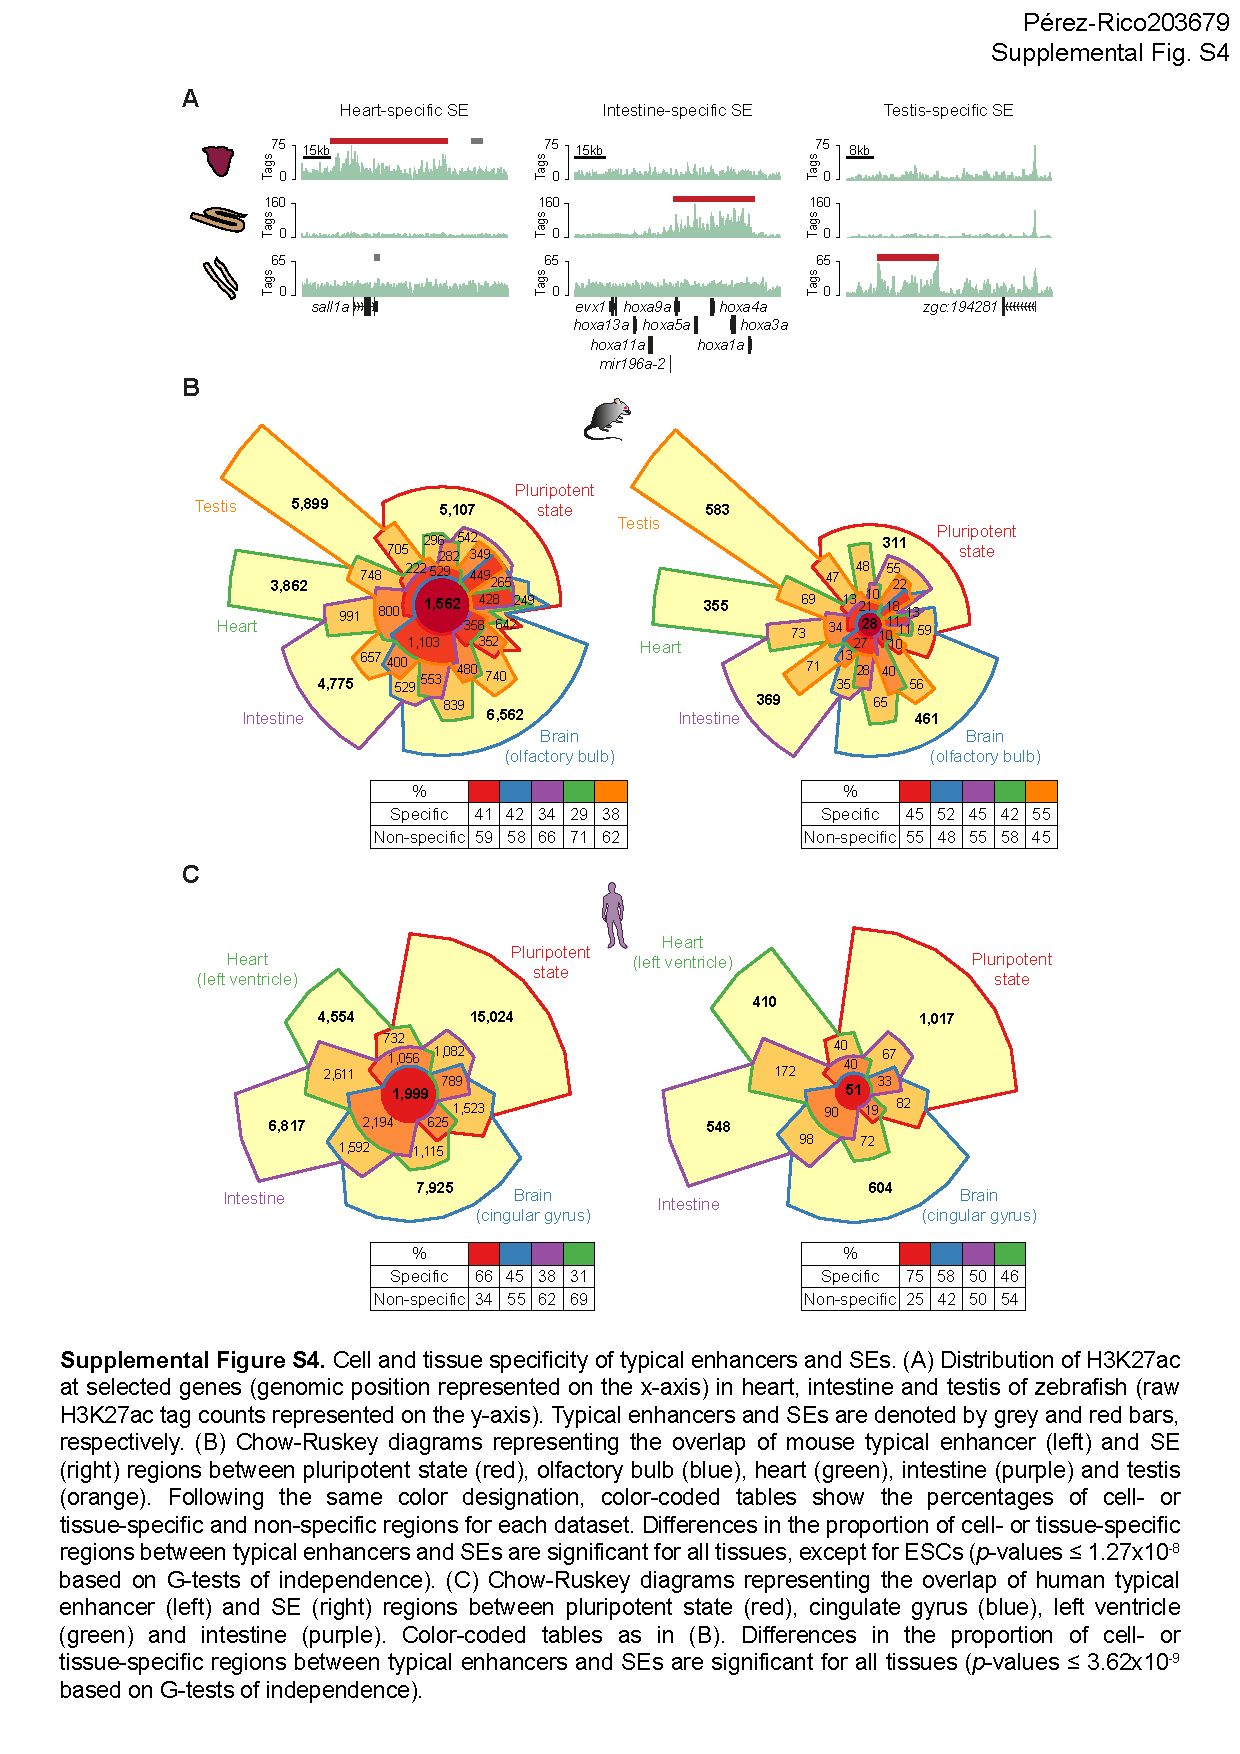
\includepdf[pages=-, pagecommand={\thispagestyle{plain}}, scale=0.8]{GenomeRes_2017/Supplemental_Fig_S4.pdf}

		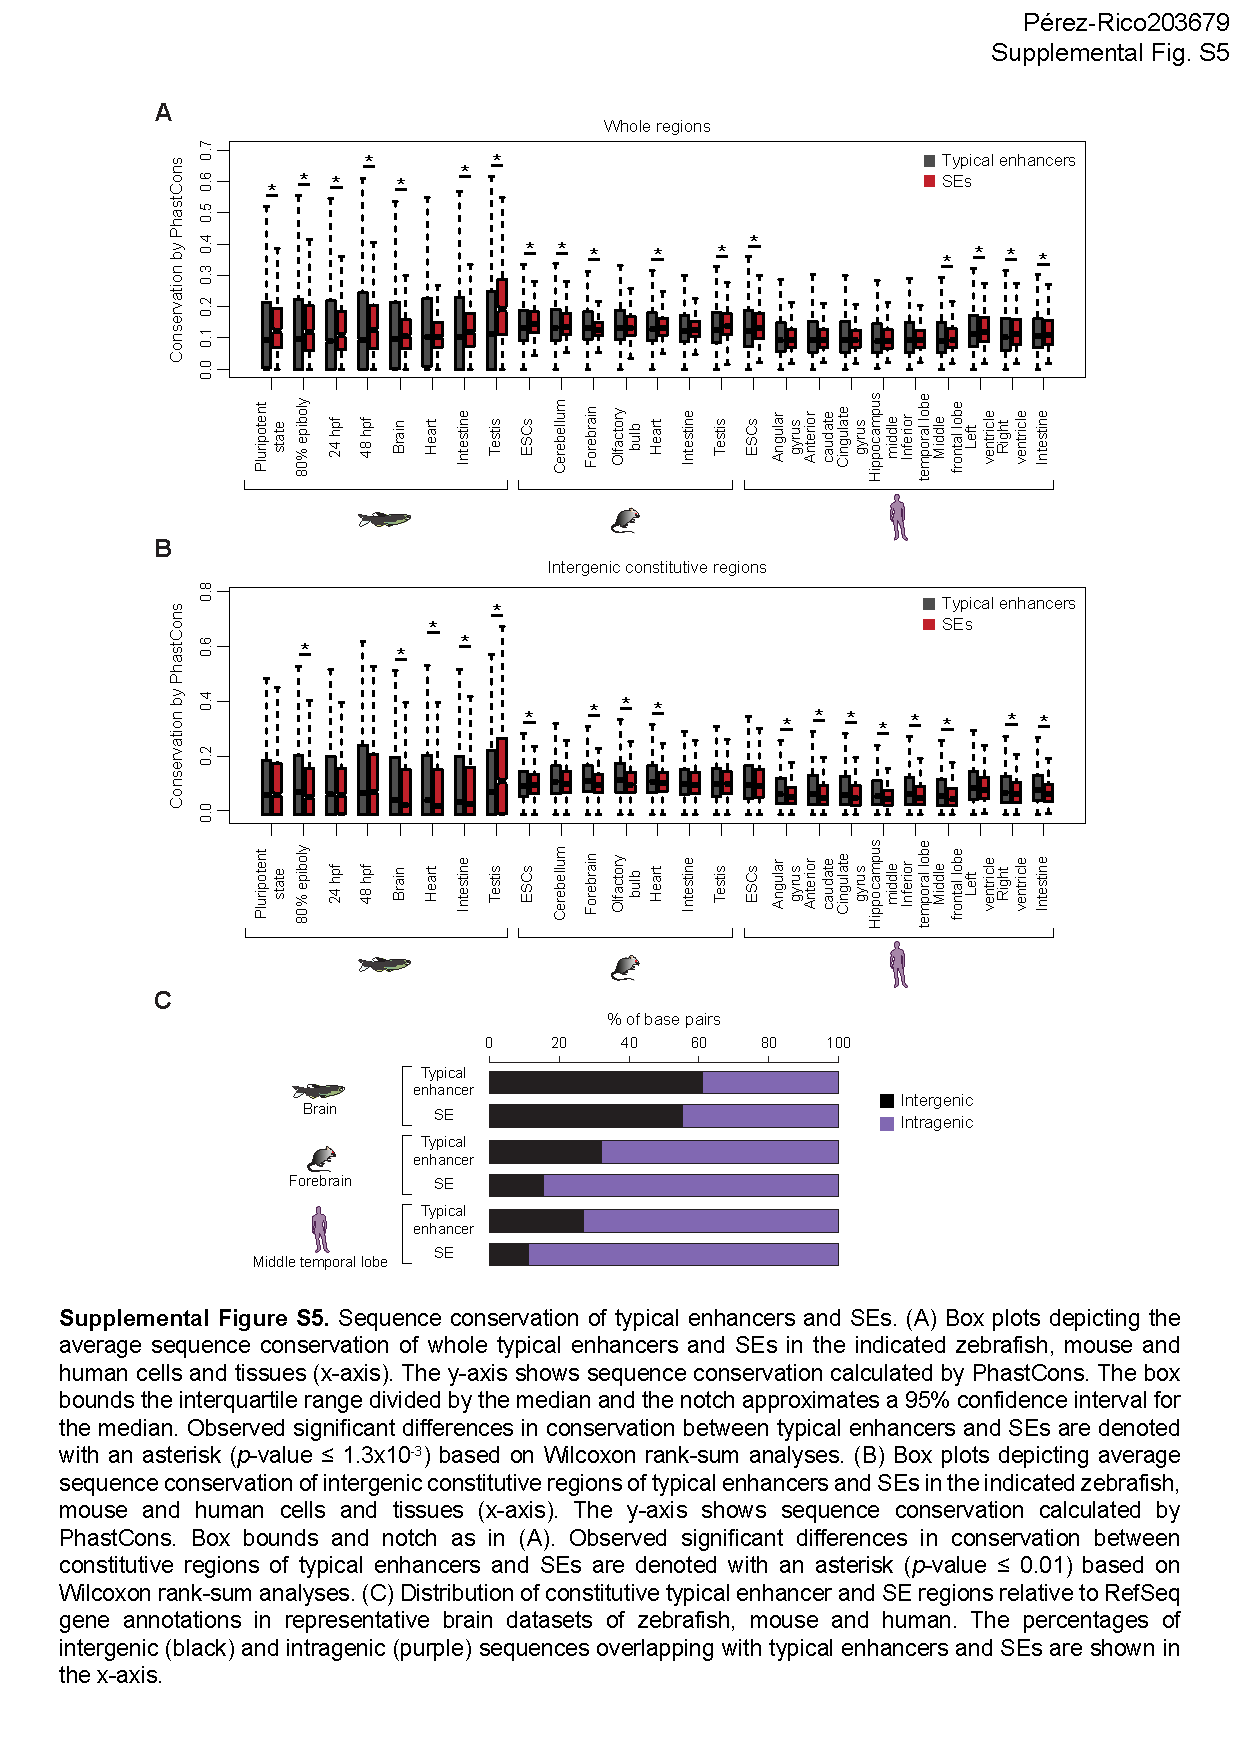
\includepdf[pages=-, pagecommand={\thispagestyle{plain}}, scale=0.8]{GenomeRes_2017/Supplemental_Fig_S5.pdf}

		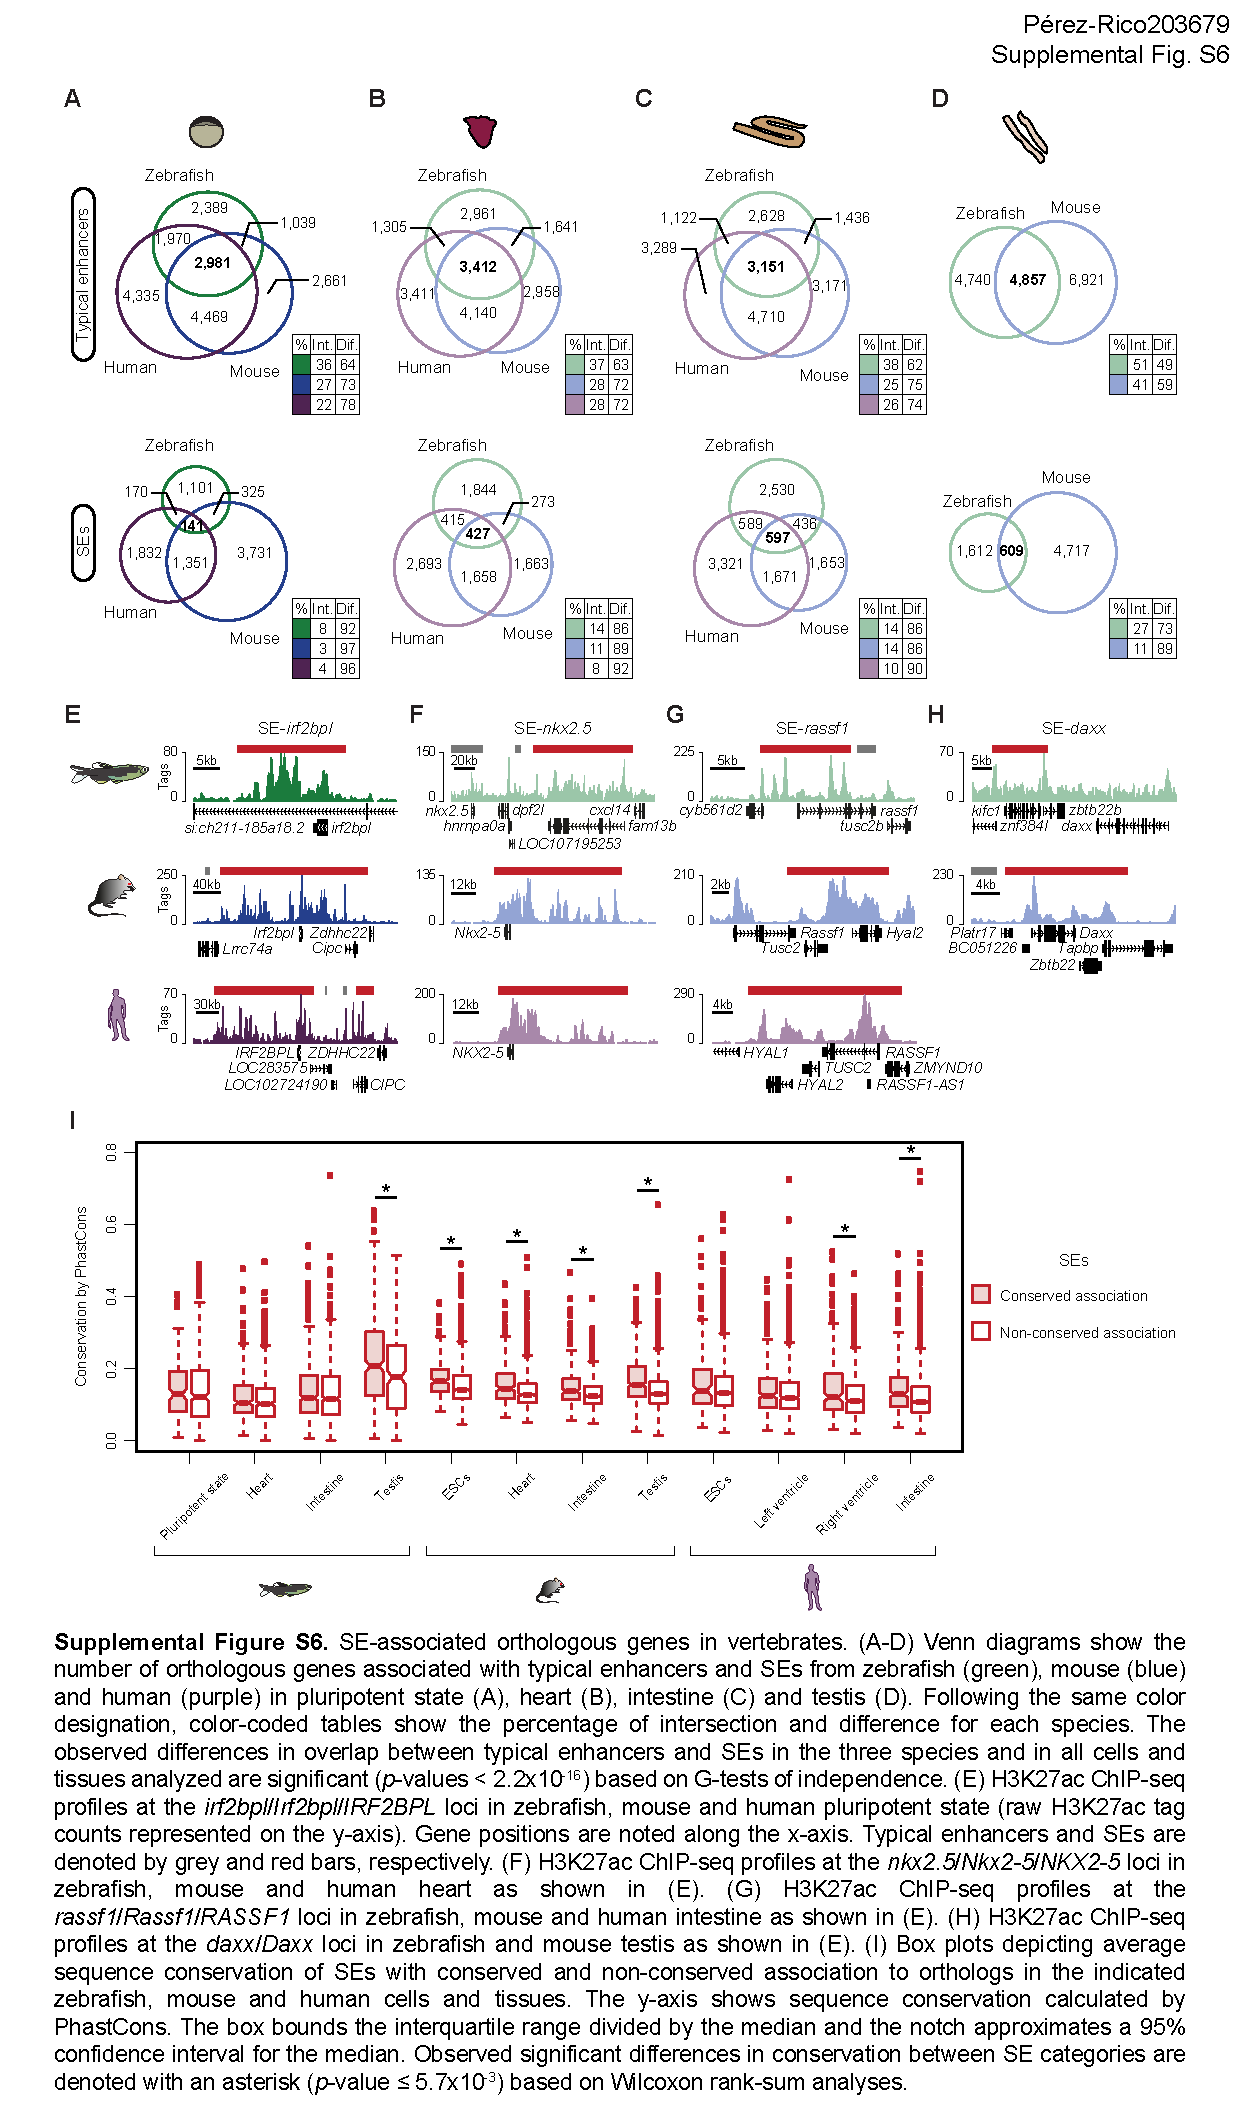
\includepdf[pages=-, pagecommand={\thispagestyle{plain}}, scale=0.8]{GenomeRes_2017/Supplemental_Fig_S6.pdf}

		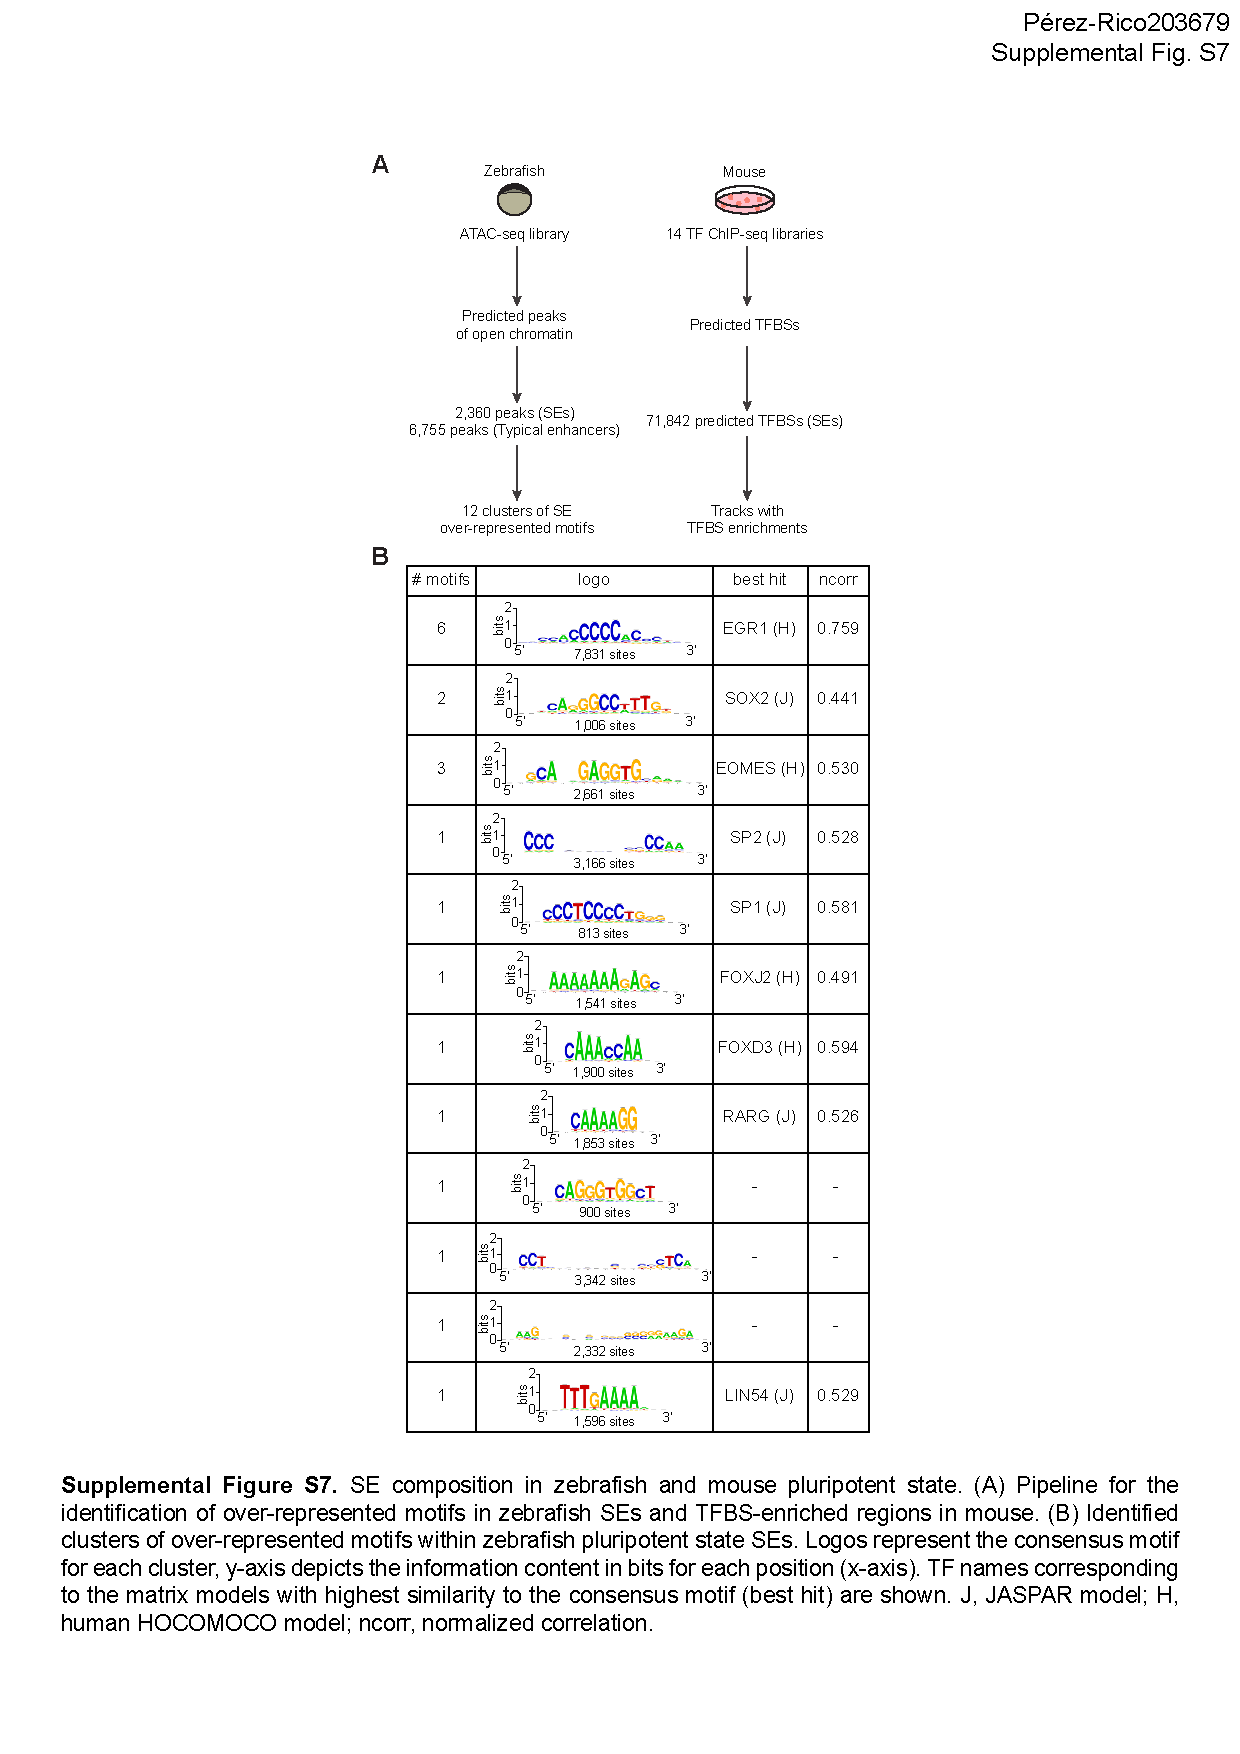
\includepdf[pages=-, pagecommand={\thispagestyle{plain}}, scale=0.8]{GenomeRes_2017/Supplemental_Fig_S7.pdf}

		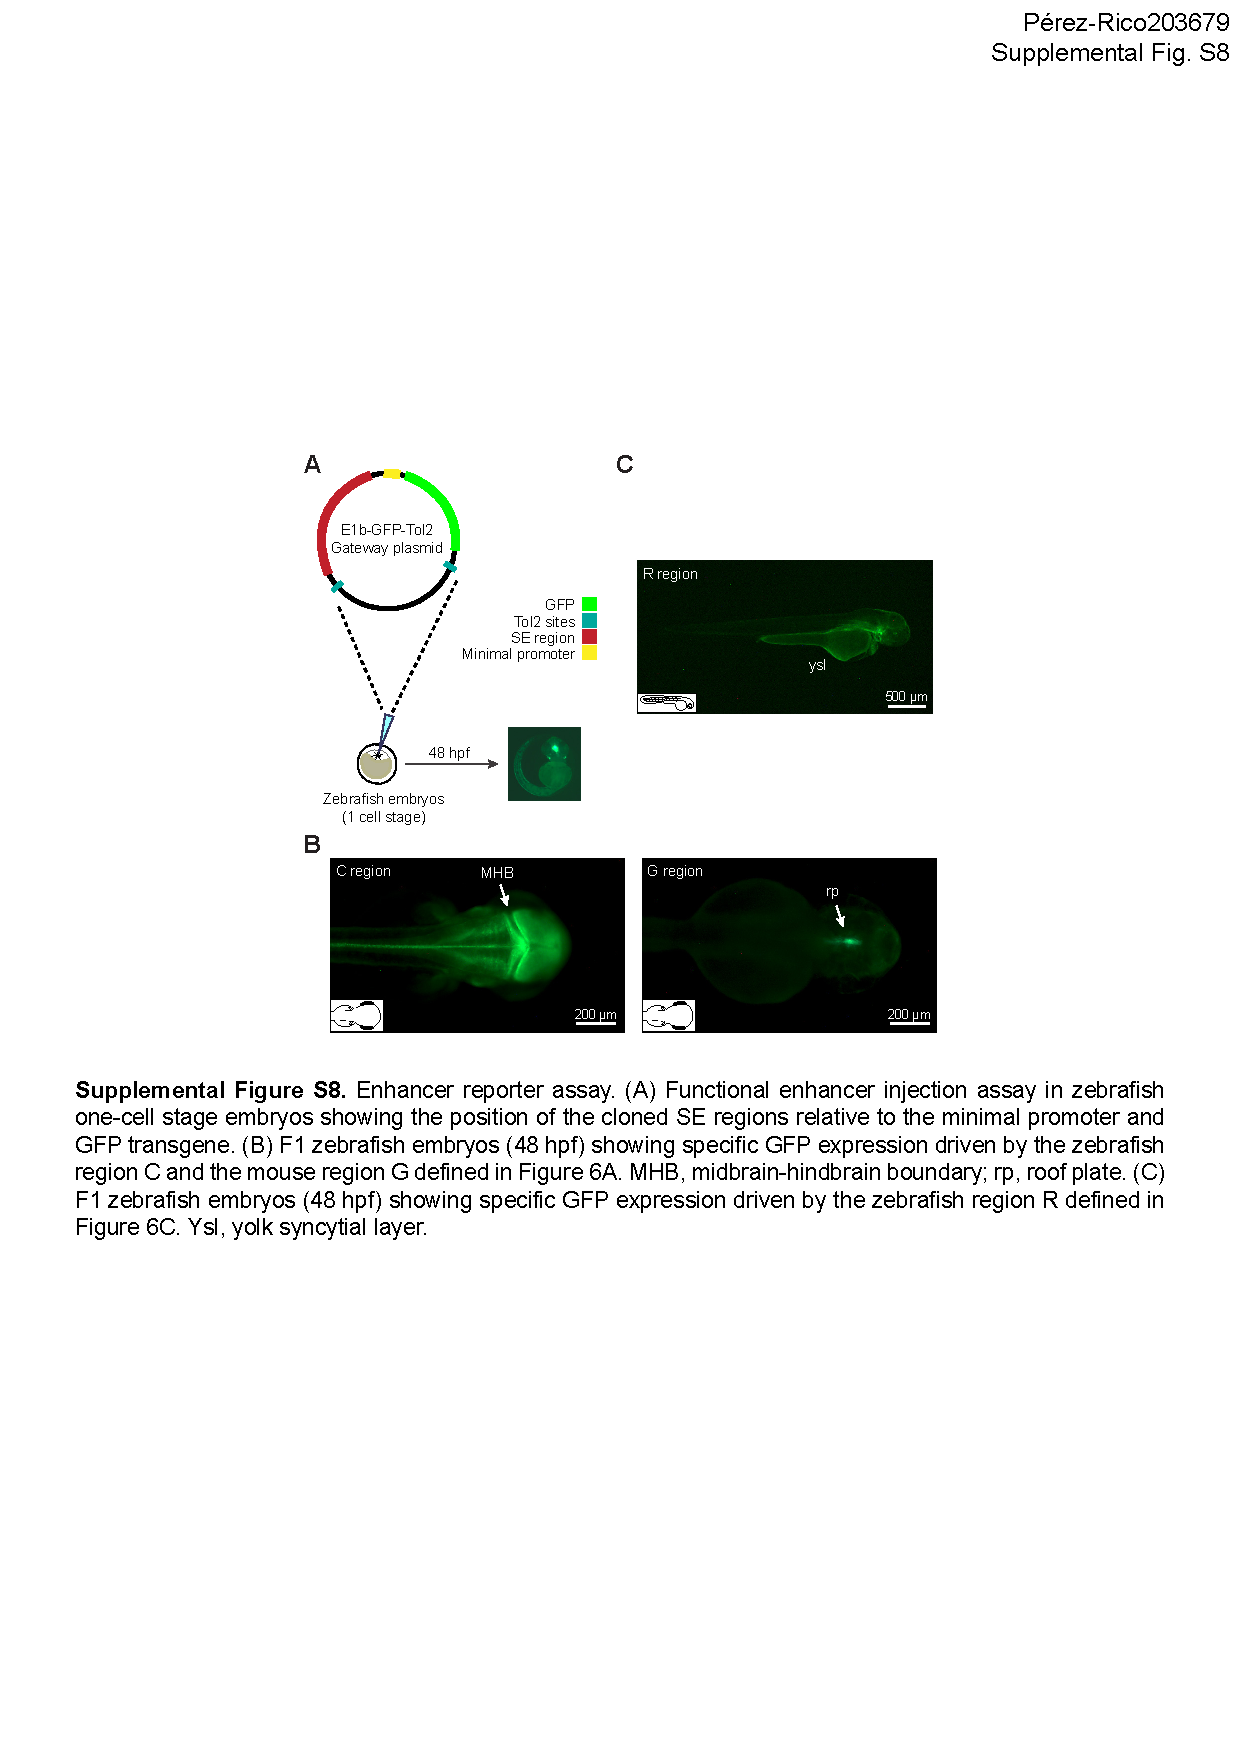
\includepdf[pages=-, pagecommand={\thispagestyle{plain}}, scale=0.8]{GenomeRes_2017/Supplemental_Fig_S8.pdf}

	\section{\textit{In vivo} analysis of CTCF functions in the zebrafish genome}

		The architectural protein CTCF has emerged as a main regulator of the 3D genome organization in mammals. However, the functions of CTCF have been evaluated in a limited number of bilaterian organisms and studies in \textit{Drosophila} have indicated the different roles of CTCF in the genome organization of flies and mammals. Hence, to contribute to the determination of CTCF functions in a phylogenetically distant vertebrate from mammals, genome-wide binding of CTCF has been evaluated for the first time in zebrafish. By integrating additional public genomic data two of the functions of CTCF have been examined.\\ 

		\subsection{Main findings}

			CTCF binding to the zebrafish genome has been difficult to assess, due to the lack of ChIP-seq grade quality antibodies. To overcome this caveat, the CRISPR/Cas9 technology was used to insert an HA-tag in-frame with the coding sequence of \textit{ctcf}. Using this transgenic fish line two biological replicates of CTCF ChIP-seq were generated. ChIP-seq replicates show high correlation and the identified peaks have higher sequence conservation than randomly distributed controls.\\

			Analysis of histone marks over the CTCF peaks show a general enrichment on marks associated with promoters and enhancers. Similarly to described binding sites of CTCF in other vertebrates, extensive motifs of CTCF binding can be identified in a fraction of the CTCF peaks. In addition, repeats enriched on CTCF binding sites were determined, suggesting which sequences could be contributing in the expansion of CTCF sites in this species.\\

			Most of the CTCF peaks localize at intronic and intergenic regions, but there is a small fraction of them that overlaps promoters. For those peaks located in promoter regions, a positive association between the abundance of CTCF and gene expression was identified. Analysis of DNA accessibility supports a mechanism in which CTCF facilitates the establishment of nucleosome free regions in promoters that results in high levels of expression.\\

			Finally, to assess the role of CTCF in the genome organization in zebrafish, Hi-C maps were analyzed. Only a small percentage of CTCF sites is located at contact domain boundaries and, in contrast to its distribution in mammals, CTCF is not enriched at contact domain boundaries of zebrafish embryos. Conversely, marks associated with active transcription show enrichment at boundaries.\\

			In conclusion, the results here presented support the hypothesis of the CTCF code and suggest differences in the relevance of CTCF in the regulation of genome organization in vertebrates. The establishment of this transgenic line opens the possibility to study in more depth the functions of CTCF in zebrafish and therefore, to evaluate its functions in less heterogenic samples.\\


		\includepdf[pages=-, pagecommand={\thispagestyle{plain}}, scale=0.95]{CTCF_paper/Manuscript_CTCF_embryo_analyses_FINAL_THESIS.pdf}

		\setcounter{figure}{0}

		\begin{figure}[h!]
			\centering
			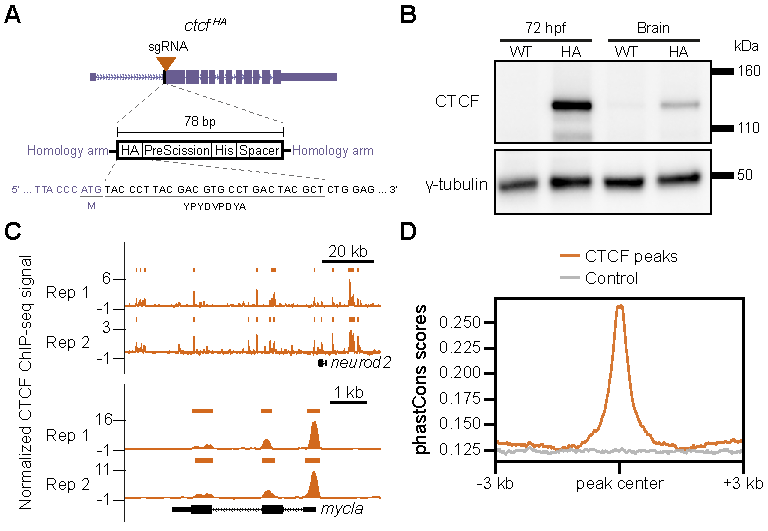
\includegraphics{CTCF_paper/Figure_1.pdf}
  			\caption[one]{Identification of CTCF binding in zebrafish.
(A) Scheme of the \textit{ctcf\textsuperscript{HA}} locus showing the insert used for tagging and the sgRNA site. Sequences at the bottom represent the partial ssDNA oligo corresponding to the HA-tag plus flanking nucleotides and the HA-tag peptide. Sequence in bold is part of the coding sequence; ATG, start codon.
(B) Western blot analysis of wild type (WT) and \textit{ctcf\textsuperscript{HA/HA}} (HA) embryos and adult brains showing specific detection of HA-CTCF in the transgenic line. Molecular weights are indicated on the right.
(C) Tracks showing examples of CTCF peaks in two genomic locations. Displayed signal distributions and peaks correspond to biological replicates (Rep 1, Rep2). Signal is represented on the \textit{y}-axis as -$\log_{10}$ (p-value) of the CTCF ChIP-seq signal.
(D) Distribution of the average sequence conservation of CTCF peaks and control regions using as reference point peak centers.}
			\label{one}
		\end{figure}

		\newpage

		\begin{figure}[h!]
			\centering
			\includegraphics{CTCF_paper/Figure_2.pdf}
  			\caption[two]{Characterization of CTCF peaks and binding sites.
(A) Heat map profiles of four histone marks and ATAC-seq data at CTCF peaks ranked by decreasing CTCF ChIP-seq signal over the displayed region. Normalized signal is shown in FPM (fragments per million mapped fragments) for ATAC-seq and in RPKM (reads per kilobase million) for histone marks.
(B) Dendogram representing the hierarchical clustering results of CTCF and CTCFL motifs. Ncor, normalized Pearson correlation.
(C) Top, histogram showing the number of co-occurrences of the CTCF core and upstream motif at different spacing distances (6 – 25 bp). Non-significant enriched spacings are colored in grey, and enrichments are shown in pink, whereas the highest enrichments are shown in red. Bottom, inferred upstream motifs using the sequences matching to the reference motif at the indicated distances from the CTCF core motif.
(D) Proportion of the top five DNA transposon types enriched on CTCF binding sites. For control regions the mean and the standard deviation (error bars) calculated by bootstrap analyses are shown.}
			\label{two}
		\end{figure}

		\newpage

		\begin{figure}[h!]
			\centering
			\includegraphics{CTCF_paper/Figure_3.pdf}
  			\caption[three]{High CTCF binding at promoters associates with high expression levels.
(A) Distribution of CTCF peaks in different categories of genomic regions. Percentages correspond to the percentage of CTCF peaks in chromosomes for each category.
(B) Average CTCF ChIP-seq signal profiles over the TSS region of genes stratified based on the score of CTCF peaks on their promoters (Low, Medium, High) and genes with no CTCF peaks (No peak).
(C) Contingency tables showing the number of gene promoters for each of the three defined categories (color-coded as in B) that contain a CTCF motif irrespectively of its orientation (top) and in the same orientation than transcription (bottom).
(D) Expression of the stratified gene categories and genes without CTCF peaks at promoters. Observed differences in the distributions are denoted as significant (*) and non-significant (n.s.) according to two-sided Wilcoxon rank-sum test ($p-value \le 1.5x10-5$).
(E) Average ATAC-seq signal profiles over the TSS region of genes stratified based on the score of CTCF peaks on their promoters.
(F-I) Average ChIP-seq signal profiles of (F) H3K4me1, (G) H3K4me3, (H) H3K27ac and (I) H3K36me3 over gene bodies and flanking sequence of the three categories of genes with CTCF bound at promoters.}
			\label{three}
		\end{figure}

		\newpage

		\begin{figure}[h!]
			\centering
			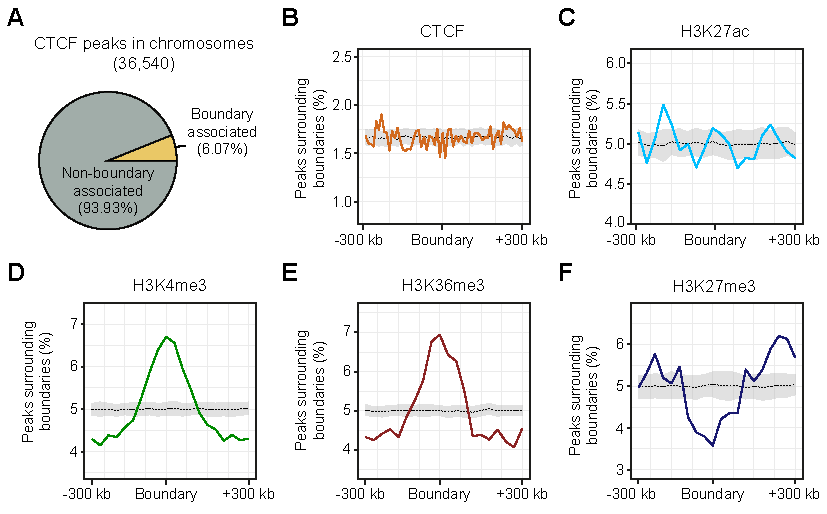
\includegraphics{CTCF_paper/Figure_4.pdf}
  			\caption[three]{Active chromatin marks, but no CTCF, are enriched at domain boundaries.
(A) Classification of CTCF peaks in chromosomes relative to contact domain boundaries.
(B) Distribution of CTCF peaks (orange) along 600 kb regions centered on contact domain boundaries (\textit{x}-axis). The \textit{y}-axis shows the percentage of total peak counts in the 600 kb region located at each genomic position. The dash line represents the mean background distribution and the grey ribbon depicts the $\pm$ 1 standard deviation range from the mean.
(C-F) Distribution of significant (C) H3K27ac, (D) H3K4me3, (E) H3K36me3 and (F) H3K27me3 peaks along contact boundary regions as described for B.}
			\label{four}
		\end{figure}


		\newpage

		\renewcommand{\figurename}{Supplemental Figure}
		\setcounter{figure}{0}

		\begin{figure}[h!]
			\centering
			\includegraphics[width=14cm,height=12cm]{CTCF_paper/Figure_S1.pdf}
  			\caption[five]{Characterization of the \textit{ctcf\textsuperscript{HA}} line.
(A) Images of wild type (WT) and \textit{ctcf\textsuperscript{HA/HA}} embryos during early development. Scale bars for each stage are displayed. Hfp, hours post-fertilization.
(B) Images of wild type (WT) and \textit{ctcf\textsuperscript{HA/HA}} adult fish. Representative fish of each sex and genotype are shown. Scale bars for each genotype are displayed.
(C) Whole gel of the Western blot shown on Fig. 1B and performed using wild type (WT) and \textit{ctcf\textsuperscript{HA/HA}} (HA) embryos and adult brains. Molecular weights are indicated on the left.}
			\label{five}
		\end{figure}

		\newpage

		\begin{figure}[h!]
			\centering
			\includegraphics[width=14cm,height=14cm]{CTCF_paper/Figure_S2.pdf}
  			\caption[six]{Identification of CTCF binding in zebrafish.
(A) Circos plot showing the average CTCF ChIP-seq signal of the two biological replicates in all chromosomes binned in 1 Mb windows. The CTCF peak enrichment track represents enrichment of CTCF peaks identified with combined replicates in 1 Mb windows. Zoom-in of chromosome 15 is displayed.
(B) Correlation between CTCF ChIP-seq biological replicates. In the scatter plot each dot represents one 1Mb bin and the axes correspond to the average signals in replicate 1 (\textit{y}-axis) and replicate 2 (\textit{x}-axis).
(C) Genome track showing the distributions of CTCF signal of biological replicates at the \textit{ctcf} locus.
(D) Distribution of the average sequence conservation of non-exonic CTCF peaks and control regions using as reference point the center of peaks and controls.}
			\label{six}
		\end{figure}

		\newpage

		\begin{figure}[h!]
			\centering
			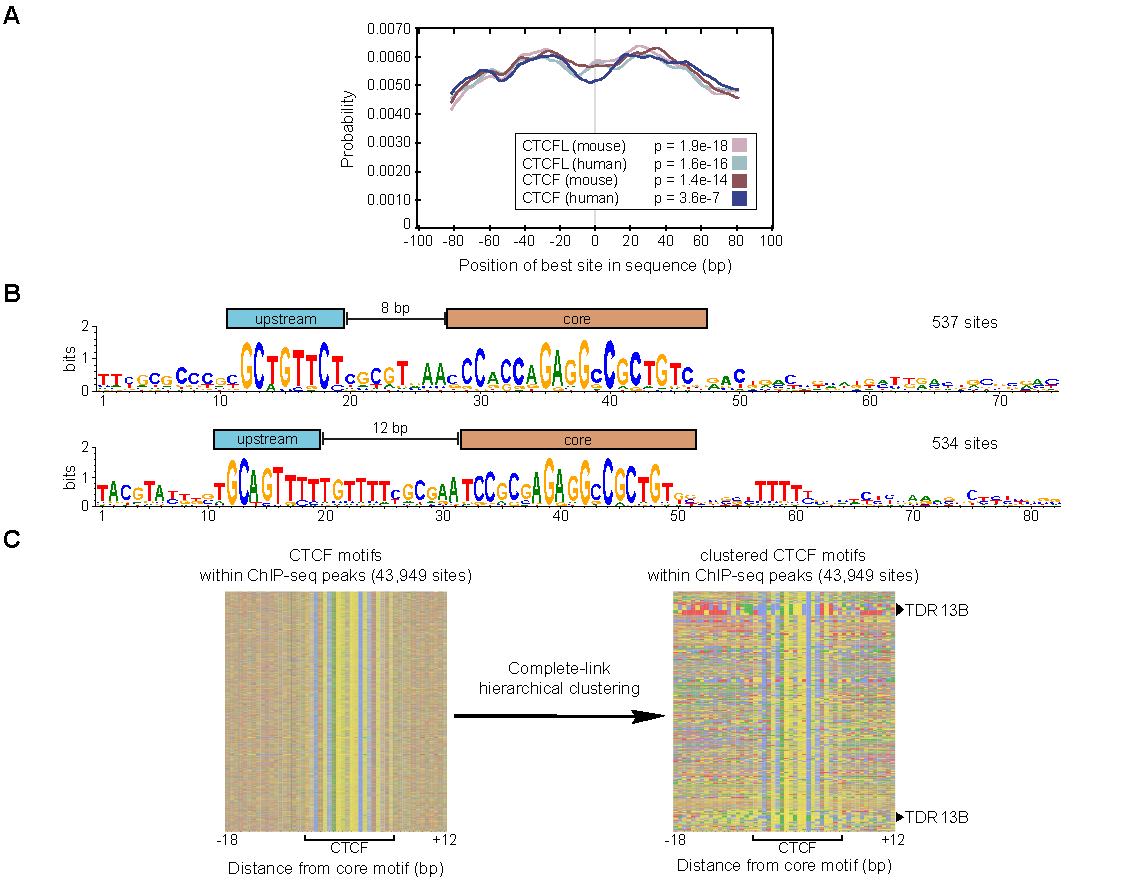
\includegraphics[width=14cm,height=13cm]{CTCF_paper/Figure_S3.pdf}
  			\caption[seven]{Analysis of CTCF binding sites.
(A) Probability distribution of the best motif matches per CTCF peak sequence calculated for the four indicated motifs. P-values support the central enrichment of the motifs.
(B) Extended motif logos for the sequences containing matches to the CTCF core and upstream motifs at spacing distances of 8 (top) and 12 bp (bottom). The number of sequences used to generate the logos is shown.
(C)  Left, color chart representing all the sequences with CTCF sites centered on the region matching to the zebrafish CTCF motif. Right, color chart with the same sequences clustered by edit distances. Clustered sequences indicating the enrichment on TDR13B repeats are indicated with triangles. Nucleotides are represented as follows: A = green, T = red, C = blue, G = yellow.}
			\label{seven}
		\end{figure}

		\newpage

		\begin{figure}[h!]
			\centering
			\includegraphics[width=14cm,height=16cm]{CTCF_paper/Figure_S4.pdf}
  			\caption[eight]{Analysis of promoters with and without CTCF peaks.
(A) Profiles and heat maps of ATAC-seq signal in promoters that do not contain a CTCF peak. Promoters were assigned to eight clusters using k-means.
(B) Genome browser showing strand-specific RNA-seq, CTCF ChIP-seq, ATAC-seq and histone ChIP-seq signal around the \textit{pbx4} gene, which promoter has a highly-bound CTCF peak.
(C) Average H3K27me3 ChIP-seq signal profiles over gene bodies and flanking sequence of the three categories of genes with CTCF bound at promoters.
(D) Average H3K27me3 ChIP-seq signal profiles over gene bodies and flanking sequence of genes without CTCF peaks at promoters.
(E) Contingency table of promoters showing their classification based on the presence/absence of CTCF peaks and their bivalency status. The top pie chart represents all promoters classified based on bivalency status. Pie charts at the bottom represent bivalent promoters (left) and non-bivalent promoters (right) with or without CTCF peaks.}
			\label{eight}
		\end{figure}

		\newpage

		\begin{figure}[h!]
			\centering
			\includegraphics[width=14cm,height=17cm]{CTCF_paper/Figure_S5.pdf}
  			\caption[nine]{Visualization of Hi-C maps of zebrafish embryos shows Rabl configuration of chromosomes.
(A-B) Hi-C maps of zebrafish at (A) 24 hpf and (B) 4 hpf showing intra-chromosomal and inter-chromosomal interaction signal for all 25 chromosomes. Arrowheads point to representative enrichments of interaction between centromeres and telomeres.
(C) Karyotype of the zebrafish chromosomes showing the locations of the intersections between the two strong diagonals visualized on the Hi-C maps (red) and centromeres (blue).
(D) Distribution of CTCF motifs (orange) along 600 kb regions centered on contact domain boundaries (\textit{x}-axis). The \textit{y}-axis shows the percentage of total peak counts in the 600 kb region located at each genomic position. The dash line represents the mean background distribution and the grey ribbon depicts the $\pm$ 1 standard deviation range from the mean.}
			\label{nine}
		\end{figure}

		\newpage

		\includepdf[pages=-, pagecommand={\thispagestyle{plain}}, scale=0.8]{CTCF_paper/Supplemental_File_S1.pdf}

		\includepdf[pages=-, pagecommand={\thispagestyle{plain}}, scale=0.8]{CTCF_paper/Supplemental_Table_S1.pdf}

		\includepdf[pages=-, pagecommand={\thispagestyle{plain}}, scale=0.8]{CTCF_paper/Supplemental_Table_S2.pdf}


